\newpage
\chapter{Introduction}
\section{Installation}
To start your programming adventure, you must have the following setup:
\begin{itemize}
    \item Windows 10
    \item \gls{nmake} installed (Microsoft Visual-Studio C++)
\end{itemize}
We recommend CLion as IDE. Later, we will also provide the possibility to use Microsoft VisualStudio (MSVC).
\subsection{Configure CLion}
Once you've installed the prerequisites, you have to configure CLion to be able to build the project.
In a first step, open CLion and press 'File - New Project'.
Select the top level CMakeLists.txt file and open it as a project.
Now, we can start with the build environment.
\begin{itemize}
    \item Open 'File - Settings'
    \item Navigate to 'Build, Execution, Deployment'
    \item Select 'Toolchains'
    \item Check if a toolchain called something like 'Visual Studio' is available.
    If yes, you don't have to go further with these steps.
    \item Press the 'Add' Button on the upper left corner
    \item Now you have to select the environment.Take a look at the following picture.
    You require at least a CMake-Version of 3.15 (The bundled one should be fine).\par
    \begin{minipage}{\linewidth}
        \centering
        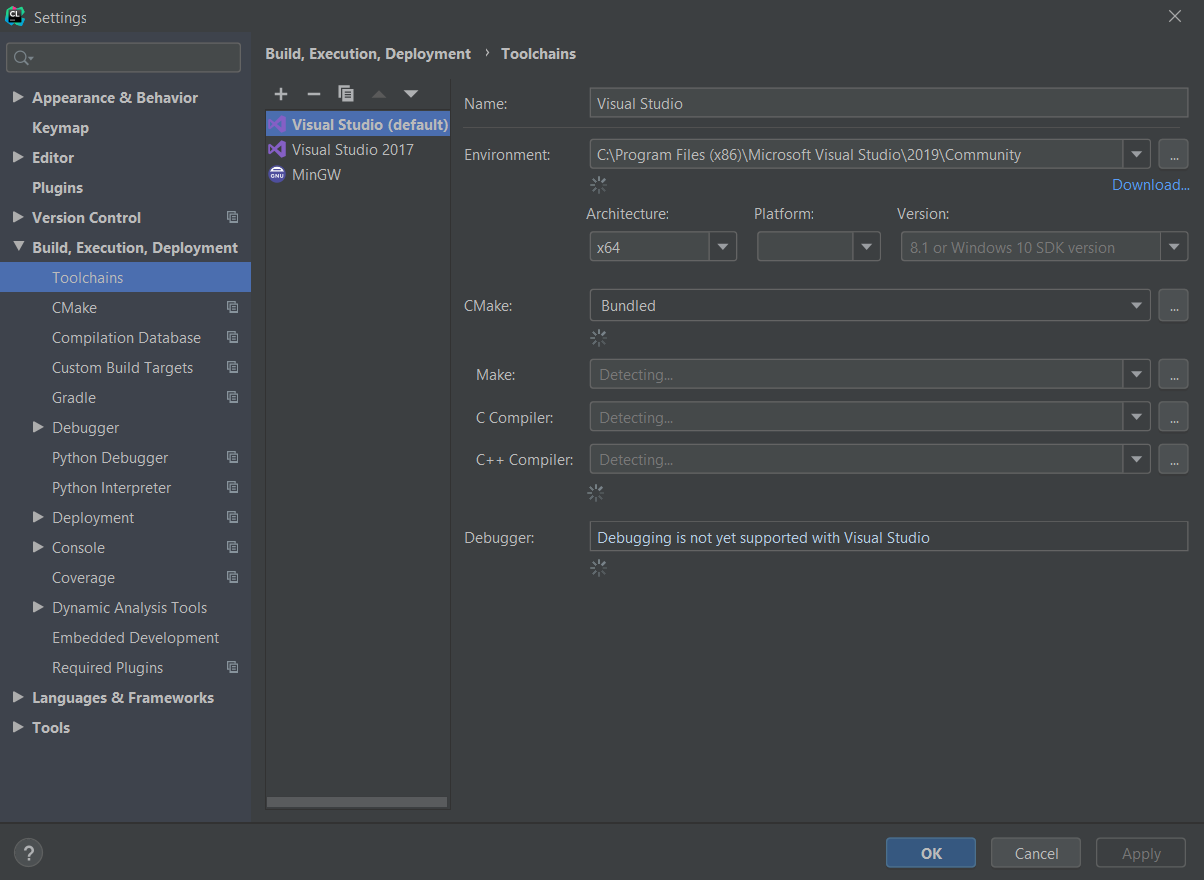
\includegraphics[width=0.6\textwidth]{./chapter_01/resources/00_clion_configure_toolchain.png}
        \captionof{figure}{CLion toolchain configuration}
    \end{minipage}
\end{itemize}
Now you are able to build the project in 'Debug' mode. This means, that in every library or executable file some additional
code gets added to debug your application. This makes your binaries approximatly ten times slower. If you want to build
a project in 'Release' mode, you have to do the following steps.
\begin{itemize}
    \item Open 'File - Settings'
    \item Navigate to 'Build, Execution, Deployment'
    \item Select 'CMake'
    \item Check if a profile called 'Release' is available. If yes, you don't have to go further with these steps.
    \item Press the 'Add' Button on the upper left corner
    \item Name it 'Release' if it is not already named like that.
\end{itemize}
Wait till CMake has imported the changes. After the CMake import, have a look on the upper right corner of the application.
You see a green hammer symbol. Next to that, there is a dropdown where you can select the 'targets'.
The release mode is printed behind the target. Per default, this is 'Debug' (you can change that in the settings).
If you open this dropdown, you can see, that you're able to switch between these modes and you can select all
targets. A target in this context means in the most cases a build of a library or executable file. But it can also
be some special stuff like copying files to directory. You should see at least the following targets:
\begin{description}
    \item[app\textunderscore basic] The main application (You have to press the green play-button behind the dropdown.)
    \item[copy\textunderscore libraries] Copies the external shared libs to the correct place.
    \item[copy\textunderscore modules] Copies the modules to the correct place.
    \item[00\textunderscore base\textunderscore module] Contains all basic setup stuff.
    \item[01\textunderscore keyboard\textunderscore module] The first set of exercises.
    \item[01\textunderscore keyboard\textunderscore module\textunderscore solution] The first set of solutions.
    \item[gmock] Test libs used by external project.
    \item[gmock\textunderscore main] Test libs used by external project.
    \item[gtest] Test libs used by external project.
    \item[gtest\textunderscore main] Test libs used by external project.
    \item[spdlog] Logging libs used by external project.
    \item[tello] Library to interact with your Tello-EDU drone.
    \item[tello\textunderscore test] Test executable used by external project.
    \item[copy\textunderscore shared\textunderscore test\textunderscore libraries] Target of external project
    \item[shared\textunderscore linking\textunderscore test] Target of external project.
\end{description}
\newpage
To compile a target, select it in the dropdown and press the green hammer next to it.
For the first time, you should build the following targets:
\begin{itemize}
    \item app\textunderscore basic
    \item 00\textunderscore base\textunderscore module
    \item 01\textunderscore keyboard\textunderscore module
\end{itemize}
The builds should run without any exceptions.
Now you can start your Tello-EDU drone. Put it somewhere on the ground, where it has some space around it.
Then select the WIFI-Settings on your computer and change into your Tello-EDU WLAN. The drone should blink yellow, this
means, it waits to a connection.\newline
Then select the target 'app\textunderscore basic' and press the play button. To test your environment, press the
'Take off' button on the center of the screen. If the drone is flying, you've done all correctly and you are
able to start (press the button again to land the drone). Congratulations, you can close the application.
\section{Architecture}
The project consists of an executable (app\textunderscore basic), which basically just loads all the plugins.
The plugins are the essential parts. They contain the exercises and solutions. Each plugin is a self-contained application,
which is specialized for a specific use-case e.g. flying with arrow keys, fly by recognitions etc.
\begin{figure}[H]
    \centering
    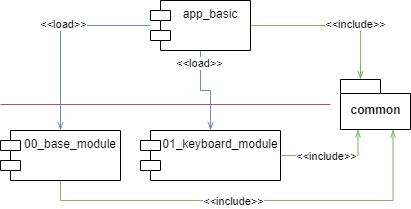
\includegraphics[width=0.6\textwidth]{./chapter_01/resources/01_architecture.png}
    \captionof{figure}{Architecture}usw.
\end{figure}
When you added your changes to one of the modules, select that module in the target dropdown, rebuild it and then
start the target 'app\textunderscore basic' to see your changes. For a reference implementation, have a look at the solutions.
They are postfixed with '\textunderscore solution'. Each excercise section in this document has a solution section at
the end of a chapter. If you're surce you have the correct solution, take a look.\newline
And now we wish you a lot of fun.